\documentclass[10pt,aspectratio=169,t]{ctexbeamer}

\useoutertheme[subsection=false]{smoothbars}
\usefonttheme[stillsansseriflarge]{serif}
\useinnertheme{circles}
\usecolortheme{spruce}

\usepackage{hyperref}
\usepackage{multicol,calligra}
\usepackage{tikz}
\usepackage{bm}
\usepackage{amsfonts} 
\usepackage{ragged2e}
\usepackage{parskip}
\usepackage{graphicx}
\usepackage{wrapfig}
\apptocmd{\frame}{}{\justifying}{} % Allow optional arguments after frame.
\usepackage{amsmath,amssymb}
\usepackage{tabularx}% 自动调整表格宽度
\usepackage{booktabs}% 制作专业的三线表 提供了\toprule（顶线）、\midrule（中线）和 \bottomrule底线命令。
\usepackage{graphicx}% 插入与处理图形 它的核心命令是 \includegraphics。
\usepackage{multirow}% 合并多行单元格 负责表格的纵向结构，实现跨行合并。 提供了 \multirow 命令
\usepackage{colortbl}
\usepackage{caption}
\captionsetup[figure]{name=图}
\setbeamertemplate{caption}[numbered] % 图形自动编号
\linespread{1.2}% 修改全文行距
\usepackage{pgfplots}
\pgfplotsset{compat=1.18}
\setbeamertemplate{theorems}[numbered] 
\usepackage{xcolor}

% ---- 思源字体 ----
\setCJKmainfont{Source Han Serif SC}[BoldFont={Source Han Serif SC Bold}]
\setCJKsansfont{Source Han Sans SC}[BoldFont={Source Han Sans SC Bold}]

\definecolor{xyyg}{cmyk}{0,1,1,0.45}
\definecolor{xyyg_gold}{cmyk}{0,0.35,0.75,0.05}
\definecolor{xyyg_blue}{cmyk}{0.6,0.35,0.0,0.4}
\definecolor{xyyg_darkblue}{cmyk}{1.0,0.6,0.0,0.5}
\definecolor{xyyg_gray}{cmyk}{0.0,0.0,0.08,0.55}
\definecolor{xyyg_dirt}{cmyk}{0.0,0.2,0.35,0.3}
\definecolor{xyyg_orange}{cmyk}{0.0,0.7,1.0,0.0}
\definecolor{xyyg_green}{cmyk}{0.2,0.0,1.0,0.15}
\definecolor{xyyg_darkgreen}{cmyk}{0.6,0.5,1.0,0.45}
\definecolor{pantone_gold}{RGB}{135,103,79}
\definecolor{pantone_silver}{RGB}{138,141,143}
\definecolor{WM_Gold}{cmyk}{0.09,0.29,0.66,0.24}
\definecolor{accent}{RGB}{196,60,50}
\definecolor{dotpink}{RGB}{214,60,120}
% =========设置footline==============
\setbeamertemplate{footline}{%
	\leavevmode%  <-- 【关键修复】强制进入水平模式，防止报错
	\hbox{%
		% 左侧 30%：作者
		\begin{beamercolorbox}[wd=0.3\paperwidth, ht=2.5ex, dp=1ex, leftskip=.3cm,center]{footleft}%
			\usebeamerfont{author in head/foot}\insertshortauthor%
		\end{beamercolorbox}%		
		% 中间 50%：标题（居中）
		\begin{beamercolorbox}[wd=0.5\paperwidth, ht=2.5ex, dp=1ex, center]{footmid}%
			\usebeamerfont{title in head/foot}\insertshorttitle%
		\end{beamercolorbox}%		
		% 右侧 20%：页码（右对齐）
		\begin{beamercolorbox}[wd=0.2\paperwidth, ht=2.5ex, dp=1ex, right, rightskip=.3cm]{footright}%
			\usebeamerfont{frame number}\insertframenumber~/~\inserttotalframenumber%
		\end{beamercolorbox}%
	}%
	\vskip0pt% <-- 【关键修复】消除底部多余空白
}%
% ======================================
% =============设置headline ==================
\newlength{\beamerheadheight}
\newlength{\beamertitleht}
\newlength{\beamertitledp}
\AtBeginDocument{\global\beamerheadheight=11.6pt}
\setbeamertemplate{headline}{%
	\begin{beamercolorbox}[wd=\paperwidth,colsep=0pt,ht=\beamerheadheight,dp=0.5ex,vmode]{section in head/foot}%
		\vbox to \beamerheadheight{%
			{\vskip0.52pt}%  
			\insertnavigation{\paperwidth}% 在当前页面（通常是页眉或页脚）生成并插入一条完整的“章节导航条”。
			\vss}%
	\end{beamercolorbox}%
}%
% ============== 设置frametitle =====================
\setbeamertemplate{frametitle}
{%
	\nointerlineskip %标题上方不留额外间距
	\usebeamerfont*{frametitle}%
	\settoheight{\beamertitleht}{\insertframetitle}% 测量标题文字的高度
	\settodepth{\beamertitledp}{\insertframetitle}% 测量标题文字的深度（下伸部分）
	\begin{beamercolorbox}[wd=\paperwidth,sep=0ex,ht=1em,% sep是与上面的间距
		dp=\dimexpr\beamertitledp+2pt,rightskip=2em,leftskip=0.5em\relax]{frametitle}%
		\usebeamercolor{frametitle}\strut\insertframetitle %插入标题文字（用strut保证基线一致）
	\end{beamercolorbox}%
}

%\setbeamerfont{frametitle}{series=\bfseries,size=\large}%,parent=structure}
%\setbeamerfont{footline}{series=\bfseries}
%\setbeamerfont{title}{series=\bfseries}

%\setbeamercolor{palette primary}{use=structure,fg=white,bg=structure.fg}
%\setbeamercolor{palette secondary}{use=structure,fg=white,bg=structure.fg!95!black}
%\setbeamercolor{palette tertiary}{use=structure,fg=white,bg=structure.fg!90!black}
%\setbeamercolor{palette quaternary}{fg=white,bg=structure.fg!85!black}
%\setbeamercolor{fine separation line}{}
%\setbeamercolor{item projected}{fg=white}
%\setbeamercolor{separation line}{}
\setbeamercolor{structure}{fg=xyyg}
\setbeamercolor{frametitle}{bg=white,fg=xyyg}
\setbeamercolor{title}{bg=xyyg,fg=white}
\setbeamercolor{section in head/foot}{bg=xyyg,fg=white}
\setbeamercolor{section in head/foot shaded}{bg=xyyg,fg=white!55!xyyg}
% 绑定颜色到 Beamer 模板
\setbeamercolor{footleft}{bg=xyyg, fg=white}
\setbeamercolor{footmid}{bg=xyyg!60!xyyg_orange, fg=white}
\setbeamercolor{footright}{bg=xyyg, fg=white}
%\setbeamertemplate{navigation symbols}{\insertslidenavigationsymbol,\insertframenavigationsymbol,%
%\insertsubsectionnavigationsymbol,\insertsectionnavigationsymbol,\insertdocnavigationsymbol}
\AtBeginDocument{
% 设置 alertblock 标题栏的颜色（fg=前景色，bg=背景色）
\setbeamercolor{block title alerted}{fg=white, bg=structure.fg!80}
% 设置 alertblock 正文区域的颜色
\setbeamercolor{block body alerted}{fg=black, bg=structure!10}	
\setbeamercolor{block title}{bg=xyyg,fg=white}
\setbeamercolor{block body}{bg=xyyg!10}	
\setbeamertemplate{enumerate items}[default]
\setbeamertemplate{itemize items}[ball]
}

\author[好好学习，努力向上]{} 
\title[高一数学第一章复习]{高一数学第一章复习}
\subtitle{集合与常用逻辑用语}
\institute{}
\date{2026/11/24}
\begin{document}

\begin{frame}
	\titlepage
\end{frame}

\section{第一节}
\begin{frame}{这是颜色名称}\vspace{-1em}	
	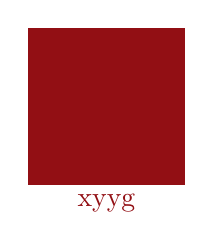
\begin{tikzpicture}
		\fill[xyyg](0,0) rectangle(2,2)node[below]at (current bounding box.south){xyyg};
	\end{tikzpicture}
	
\begin{tikzpicture}
		\fill[xyyg_dirt](0,0) rectangle(2,2)node[below]at (current bounding box.south){xyyg\_dirt};
	\end{tikzpicture}
	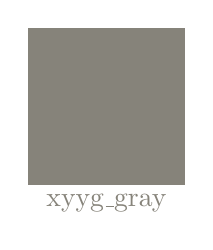
\begin{tikzpicture}
		\fill[xyyg_gray](0,0) rectangle(2,2)node[below]at (current bounding box.south){xyyg\_gray};
	\end{tikzpicture}
	
\begin{tikzpicture}
		\fill[xyyg_darkblue](0,0) rectangle(2,2)node[below]at (current bounding box.south){xyyg\_darkblue};
	\end{tikzpicture}
	
\begin{tikzpicture}
		\fill[xyyg_blue](0,0) rectangle(2,2)node[below]at (current bounding box.south){xyyg\_blue};
	\end{tikzpicture}
	
\begin{tikzpicture}
		\fill[xyyg_gold](0,0) rectangle(2,2)node[below]at (current bounding box.south){xyyg\_gold};
	\end{tikzpicture}
	
	\vspace{-1em}
	
\begin{tikzpicture}
		\fill[xyyg_orange](0,0) rectangle(2,2)node[below]at (current bounding box.south){xyyg\_orange};
	\end{tikzpicture}
	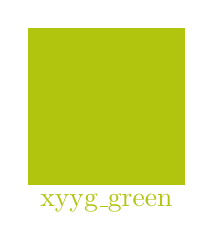
\begin{tikzpicture}
		\fill[xyyg_green](0,0) rectangle(2,2)node[below]at (current bounding box.south){xyyg\_green};
	\end{tikzpicture}
	
\begin{tikzpicture}
		\fill[xyyg_darkgreen](0,0) rectangle(2,2)node[below]at (current bounding box.south){xyyg\_darkgreen};
	\end{tikzpicture}
	
\begin{tikzpicture}
		\fill[pantone_gold](0,0) rectangle(2,2)node[below]at (current bounding box.south){pantone\_dirt};
	\end{tikzpicture}
	
\begin{tikzpicture}
		\fill[pantone_silver](0,0) rectangle(2,2)node[below]at (current bounding box.south){pantone\_silver};
	\end{tikzpicture}
	
\begin{tikzpicture}
		\fill[WM_Gold](0,0) rectangle(2,2)node[below]at (current bounding box.south){WM\_Gold};
	\end{tikzpicture}
	
	\vspace{-1em}
	
\begin{tikzpicture}
		\fill[accent](0,0) rectangle(2,2)node[below]at (current bounding box.south){accent};
	\end{tikzpicture}
	
\begin{tikzpicture}
		\fill[dotpink](0,0) rectangle(2,2)node[below]at (current bounding box.south){dotpink};
	\end{tikzpicture}
	
	
\end{frame}	

\section{第二节}
\begin{frame}
	内容...
	
\end{frame}	
\begin{frame}
	内容...
\end{frame}	
\begin{frame}
	内容...
\end{frame}	
\begin{frame}
	内容...
\end{frame}	

\section{第三节}
\begin{frame}{这是标题}
	内容...
\end{frame}	
\begin{frame}
	内容...
\end{frame}	
\begin{frame}
	内容...
\end{frame}	
\begin{frame}
	内容...
\end{frame}	

\end{document}